\documentclass{article}
\usepackage{amsmath,amsthm,amssymb}
\usepackage[T2A]{fontenc}
\usepackage[utf8]{inputenc}
\usepackage[english]{babel}
\usepackage{graphicx}
\usepackage{hyperref}
\usepackage[margin=2.5cm]{geometry}
% NB: keep babel to a single language (english). Declaring a second, "main"
% language (e.g. [english,russian]) makes babel switch \encodingdefault back
% to OT1 when \selectlanguage{english} runs, breaking every embedded Cyrillic
% string later in the document ("Command \CYRxx unavailable in encoding OT1").
% We never need babel's Russian hyphenation/typography -- the Cyrillic text
% here is only quoted/table content, so T2A + utf8 alone is enough.
% Likewise, the legacy `mathtext' package (Cyrillic-in-math support, unused
% here and unmaintained since ~2003) interacts badly with this and was removed.


\title{Length Shortcuts and Unseen Generators:\\ Detecting AI-Generated Russian Scientific Abstracts}
\author{Evgeny Polikanin}
\date{2026}


\begin{document}
\selectlanguage{english}
\maketitle
\begin{abstract}
We study the detection of machine-generated scientific abstracts in Russian on the AINL-Eval 2025 benchmark, where a system must attribute an abstract to a human, to one of three known large language models, or to an \emph{unknown} model. We compare the official TF-IDF baseline, a fine-tuned mDeBERTa-v3 encoder, zero-shot perplexity-based detectors (log-perplexity and Binoculars on Qwen3-0.6B) and a hybrid feature-based detector that stacks TF-IDF class probabilities with token-level language-model statistics and stylometric features. We additionally collect 6{,}595
new abstracts produced with the official prompt by 2025 open models (Qwen2.5-3B, Qwen3-4B-2507, Qwen3-1.7B, YandexGPT-5-Lite-8B) and use them (i) as pseudo-\emph{unknown} training data and (ii) as a held-out test of generalisation to new generators. Finally, we measure how much each detector relies on the fact that human abstracts are twice as long as generated ones by re-running all experiments on texts truncated to 40 words. All models train in under an hour on a single GPU.
Code and data: \url{https://github.com/yournickname/ainl-eval-detection}.
\end{abstract}



\section{Introduction}
Large language models (LLMs) write fluent scientific prose, and generated abstracts are increasingly submitted to journals and conferences. Reviewers and editors need tools that flag such texts, and for Russian the choice of tools and benchmarks is still small. The AINL-Eval 2025 shared task~\cite{ainleval2025} released a large corpus of Russian scientific abstracts written by humans and by several LLMs, with the explicit goal of testing generalisation to \emph{new domains} and \emph{new generators}.

Two properties of this benchmark motivate our work. First, human abstracts are on average about twice as long as generated ones (Fig.~\ref{fig:lengths}), so a detector can reach high accuracy by learning length rather than style; such shortcut learning~\cite{shortcut} would not transfer to real use, where a generator can be asked for a longer text. Second, the ``unknown'' class of the task is supposed to catch any model that is not in the training data, but the training set contains no examples of it, so participants had to rely on confidence thresholds.

Our contributions are:
\begin{enumerate}
    \item A comparison of four families of detectors on AINL-Eval 2025 under a single evaluation protocol: a lexical baseline, a fine-tuned multilingual encoder, zero-shot perplexity detectors, and a hybrid feature-based detector with a linear classifier.
    \item A small new dataset of abstracts generated by 2025 open LLMs with the official prompt. Titles and keywords, which are not distributed with AINL-Eval, are reconstructed from human abstracts with an LLM. We use part of these texts as pseudo-unknown training data and keep the rest as a held-out generator test.
    \item A length-control study: all methods are re-trained and re-evaluated on abstracts cut to their first 40 words, and we also report accuracy per length bucket.
\end{enumerate}
We deliberately do not claim a new detection algorithm: our hybrid detector combines known ingredients (GLTR-style token statistics~\cite{gltr}, Binoculars~\cite{binoculars}, Ghostbuster-style feature stacking~\cite{ghostbuster}). The focus is on what the detectors actually rely on and how they behave on generators they have not seen.

\subsection{Team}
\textbf{Evgeny Polikanin} did all parts of the project: data collection, implementation of the methods, experiments and the report.



\section{Related Work}
\label{sec:related}

\paragraph{Shared tasks and datasets.}
Detection of machine-generated text has been studied in a series of shared tasks. RuATD 2022~\cite{ruatd2022} was the first Russian benchmark: it covered several text generation tasks (translation, paraphrasing, summarisation, open generation) and 13 generators, and its binary and multi-class subtasks were evaluated by accuracy. M4~\cite{m4} and SemEval-2024 Task 8~\cite{semeval2024task8} extended the setting to many domains, generators and languages, and introduced a subtask of identifying the specific generator. In these benchmarks fine-tuned transformer encoders were the strongest single systems, while zero-shot detectors lagged behind on out-of-domain data.

AINL-Eval 2025~\cite{ainleval2025} focuses on Russian scientific abstracts. Its training set has four classes (human, GPT-4-Turbo, Gemma-2-27B, Llama-3.3-70B). The development (public test) set adds GigaChat-Lite as the unknown model, and the private test set adds DeepSeek-V3 and two unseen domains. Table~\ref{tab:leaderboard} lists the official results. The winning system, GigaCheck~\cite{gigacheck}, fine-tunes Mistral-7B with LoRA and two heads (human vs AI, and generator identification). The second team fine-tuned the classification head of YandexGPT-8B on the development phase and, on the test set, combined bag-of-words features with Binoculars scores from Gemma-2B and Llama-1B. The official TF-IDF + logistic regression baseline is strong: it is fifth on the development set and fourth on the test set, ahead of a fine-tuned BERT.

\begin{table}[tbh!]
\begin{center}
\small
\begin{tabular}{|l|l|cc|}
\hline
Team & System & Dev acc & Test acc \\
\hline
sastsy & GigaCheck (Mistral-7B, LoRA) & 0.9122 & 0.8635 \\
adugeen & YandexGPT-8B / BoW + Binoculars & 0.8696 & 0.8462 \\
Nick & n/a & 0.8245 & -- \\
vikosik3000 & n/a & 0.8164 & 0.8159 \\
Baseline & TF-IDF + LR & 0.8081 & 0.8105 \\
Baseline & BERT & 0.7903 & -- \\
\hline
\end{tabular}
\caption{Official AINL-Eval 2025 results (5-class accuracy), from~\cite{ainleval2025}. The development set is the public test set with GigaChat-Lite as the unknown model; the private test set labels are not public.}
\label{tab:leaderboard}
\end{center}
\end{table}

\paragraph{Supervised detectors.}
The most common approach is to fine-tune a pretrained encoder (RoBERTa, DeBERTa~\cite{deberta3}, XLM-R) as a text classifier, as done in LLM-DetectAIve~\cite{llmdetectaive} and in most top SemEval systems. Recent systems fine-tune decoder LLMs instead, e.g.\ GigaCheck~\cite{gigacheck}. These models reach high in-distribution accuracy but are known to overfit to the generators seen in training.

\paragraph{Zero-shot detectors.}
Zero-shot methods need no labelled data and rely on the fact that LLM outputs have high likelihood under other LLMs. The simplest detector thresholds the average token log-probability~\cite{ainleval2025}; GLTR~\cite{gltr} looks at the ranks of observed tokens. DetectGPT~\cite{detectgpt} compares the likelihood of a text with that of its perturbations, and Fast-DetectGPT~\cite{fastdetectgpt} replaces perturbations with sampling from the conditional distribution, which makes it about 300 times faster. Binoculars~\cite{binoculars} normalises the perplexity of a text by the cross-perplexity between two related models, which removes much of the dependence on the prompt and the topic; it is the strongest published zero-shot detector on English benchmarks.

\paragraph{Feature-based and hybrid detectors.}
Ghostbuster~\cite{ghostbuster} passes a text through several weak language models, builds features from the token probabilities and trains a linear classifier on top; it generalises better across domains than fine-tuned encoders. Stylometric features (lengths, punctuation, lexical diversity) are another classic signal. The second-place AINL-Eval system combined bag-of-words and Binoculars features, which is close to our hybrid detector.

\paragraph{Watermarking.}
Watermarking~\cite{watermark} embeds a detectable signal at generation time. It requires control over the generator and is not applicable to texts produced by third-party models, which is the setting of this task.



\section{Model Description}
\label{sec:model}
Our main approach is a \emph{hybrid feature-based detector}: several groups of features are computed for each abstract, concatenated, standardised, and fed to a multinomial logistic regression. Only the last step is trained on labels; all feature extractors are frozen models. Figure~\ref{fig:pipeline} shows the pipeline.

\begin{figure}[!tbh]
\centering
\fbox{\begin{tabular}{c}
abstract $x$\\[2pt]
$\downarrow$\\[2pt]
\begin{tabular}{|l|l|}
\hline
TF-IDF + LR, 5-fold out-of-fold & 4 class probabilities \\
Qwen3-0.6B-Base and Qwen3-0.6B & 12 token statistics incl.\ Binoculars \\
stylometry & 14 features \\
multilingual-e5-large (ablation only) & 1024-d embedding \\
\hline
\end{tabular}\\[2pt]
$\downarrow$\\[2pt]
concatenate, standardise $\rightarrow$ multinomial logistic regression $\rightarrow$ $p(y\mid x)$
\end{tabular}}
\caption{The hybrid detector. Only the final logistic regression is trained on the labels.}
\label{fig:pipeline}
\end{figure}

\paragraph{Language-model statistics.}
Let $x = (x_1,\dots,x_n)$ be the tokens of an abstract. We use two small models that share a tokenizer: the observer $M_o$ = Qwen3-0.6B-Base and the performer $M_p$ = Qwen3-0.6B (instruction-tuned)~\cite{qwen3}. For each position we take the next-token distributions $P_o(\cdot\mid x_{<i})$ and $P_p(\cdot\mid x_{<i})$ and compute
\begin{align}
\log \mathrm{PPL}_M(x) &= -\frac{1}{n}\sum_{i=1}^{n} \log P_M(x_i\mid x_{<i}), \\
H_M(x) &= \frac{1}{n}\sum_{i=1}^{n} \Big(-\sum_{v} P_M(v\mid x_{<i}) \log P_M(v\mid x_{<i})\Big), \\
\log \mathrm{XPPL}(x) &= \frac{1}{n}\sum_{i=1}^{n} \Big(-\sum_{v} P_o(v\mid x_{<i}) \log P_p(v\mid x_{<i})\Big), \\
B(x) &= \frac{\log \mathrm{PPL}_{p}(x)}{\log \mathrm{XPPL}(x)}.
\end{align}
$B(x)$ is the Binoculars score~\cite{binoculars}: low values indicate machine-generated text. In addition we use the standard deviation of token log-probabilities, the share of tokens that are the top-1 and top-10 predictions of the observer and the mean log-rank (as in GLTR~\cite{gltr}), and the number of tokens, 12 features in total.

\paragraph{Stylometric features.}
Numbers of words, characters and sentences; mean word length; mean and standard deviation of sentence length (in words); shares of digits, Latin letters, capital letters and punctuation among characters; commas, parentheses and dashes per word; type--token ratio. These features are cheap and directly expose the length and ``digit'' differences described in the dataset paper.

\paragraph{Lexical stacking.}
The official baseline (TF-IDF over word unigrams, logistic regression with $C=5$) is a strong detector on this data, so we include its predicted class probabilities as four features. To avoid leakage, training-set probabilities are obtained with 5-fold cross-validation (out-of-fold predictions), and for other sets the model is refitted on the full training set.

\paragraph{Sentence embeddings.}
Mean-pooled, $L_2$-normalised embeddings of multilingual-e5-large~\cite{e5} (prefix ``query: '', 512 tokens). In the ablations we find that they do not help on top of the other groups, so the final model does not use them.

\paragraph{Classifier and the unknown class.}
All non-embedding features are transformed with $\mathrm{sign}(z)\log(1+|z|)$, then all features are standardised, and a multinomial logistic regression ($C=0.5$) is trained. For the open-set 5-class task we compare two ways to predict \emph{unknown}:
\begin{enumerate}
\item \textbf{Threshold rule} of the official baseline: a model trained on the 4 known classes predicts \emph{unknown} when its maximum class probability is below $0.6$.
\item \textbf{Pseudo-unknown class}: we add texts generated by \emph{other} LLMs (Section~\ref{sec:our_data}) to the training set as a fifth class and use the argmax. The detector never sees the real unknown generator of the development set (GigaChat-Lite), so this is a fair test of whether ``other LLMs'' generalise to a new one.
\end{enumerate}



\section{Dataset}
\label{sec:dataset}

\subsection{AINL-Eval 2025}
AINL-Eval 2025~\cite{ainleval2025} contains abstracts of Russian scientific papers from 12 domains (mathematics, philology, physics, chemistry, pedagogy, IT, law, medicine, oil and gas, management, economics, biology). For each human abstract the organisers prompted each LLM with the paper title and keywords (the prompt is given in Section~\ref{sec:our_data}) and post-processed the outputs, removing artefacts and rewriting typical openings. The dataset is available on the Hugging Face Hub\footnote{\url{https://huggingface.co/datasets/iis-research-team/AINL-Eval-2025}} under the Apache-2.0 licence.

The official split has 35{,}158 training texts (4 classes, balanced), 10{,}978 development texts (5 classes, GigaChat-Lite as unknown) and 6{,}169 test texts (DeepSeek-V3 as unknown, two new domains). Gold labels of the test set are not included in the public GitHub and Hugging Face releases, so \textbf{we use the labelled development set as our test set} and compare with the development-phase leaderboard (Table~\ref{tab:leaderboard}). For model selection we hold out a stratified 10\% of the training set (\emph{val}); all models are trained on the remaining 90\% (\emph{train}). No decision was tuned on the development set. Table~\ref{tab:statistics} gives the statistics.

\begin{table}[tbh!]
\begin{center}
\begin{tabular}{|l|l|rrrr|}
\hline
Split & Class / generator & Texts & Mean words & Median words & Digits / 100 w \\
\hline
train & gemma-2-27b & 7,911 & 61.9 & 61 & 0.6 \\
 & gpt-4-turbo & 7,921 & 85.8 & 85 & 0.4 \\
 & human & 7,891 & 126.0 & 104 & 4.3 \\
 & llama-3.3-70b & 7,918 & 70.6 & 69 & 0.5 \\
\hline
val & gemma-2-27b & 879 & 62.7 & 62 & 0.6 \\
 & gpt-4-turbo & 880 & 85.4 & 85 & 0.4 \\
 & human & 877 & 120.4 & 96 & 3.9 \\
 & llama-3.3-70b & 880 & 70.8 & 69 & 0.4 \\
\hline
dev & gemma-2-27b & 2,204 & 62.1 & 61 & 0.7 \\
 & gpt-4-turbo & 2,205 & 86.1 & 85 & 0.5 \\
 & human & 2,193 & 125.0 & 102 & 4.5 \\
 & llama-3.3-70b & 2,203 & 71.1 & 70 & 0.5 \\
 & unknown & 2,173 & 49.6 & 48 & 0.8 \\
\hline
ours: pseudo-unknown & qwen2.5-3b & 2,349 & 48.8 & 48 & 0.6 \\
 & qwen3-4b-2507 & 2,352 & 75.6 & 75 & 0.7 \\
\hline
ours: held-out & human & 947 & 128.5 & 109 & 3.8 \\
 & qwen3-1.7b & 947 & 65.5 & 65 & 0.5 \\
 & yandexgpt-5-lite-8b & 947 & 48.6 & 48 & 0.6 \\
\hline
\end{tabular}

\caption{Dataset statistics: number of texts, mean and median length in words, and digits per 100 words. Train/val is our 90/10 split of the official training set; dev is the official development set, used as the test set. The last block is our collected data (Section~\ref{sec:our_data}).}
\label{tab:statistics}
\end{center}
\end{table}

\begin{figure}[!tbh]
\centering
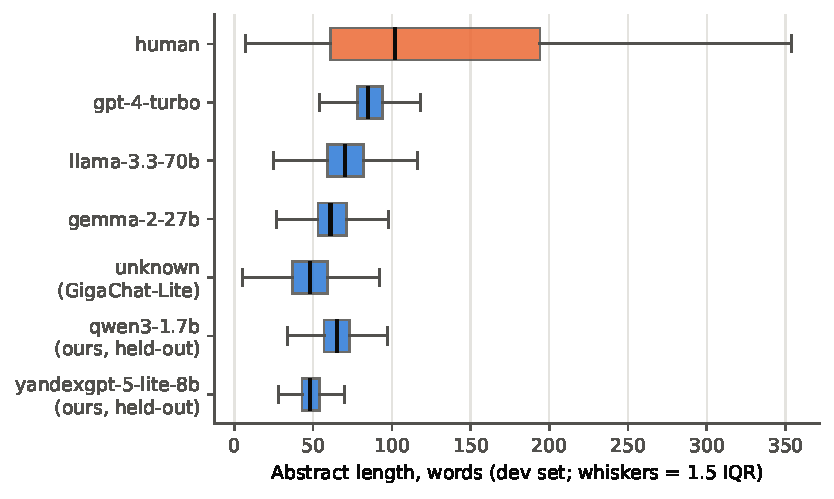
\includegraphics[width=0.75\linewidth]{figures/lengths.pdf}
\caption{Distribution of abstract lengths per class on the development set and for our held-out generators. Human abstracts are much longer and more variable.}
\label{fig:lengths}
\end{figure}

The classes differ strongly in length (Fig.~\ref{fig:lengths}): human abstracts have 125 words on average with a long tail, GPT-4-Turbo 86, Llama-3.3 71, Gemma-2 62, and GigaChat-Lite only 50. Humans also use about ten times more digits. These are real properties of generated abstracts, but they are fragile cues, which motivates our length-control experiment.

\subsection{Our collected data}
\label{sec:our_data}
To test generalisation to newer generators and to give the detectors examples of ``some other LLM'', we generated additional abstracts following the organisers' protocol as closely as possible.

\paragraph{Title and keyword reconstruction.} AINL-Eval does not include paper titles and keywords. We therefore asked Qwen2.5-3B-Instruct (greedy decoding) to produce a plausible title and 3--6 keywords for a human abstract as JSON. From 3{,}500 sampled human abstracts (2{,}500 from our train split, 1{,}000 from dev) we obtained 3{,}299 valid pairs.

\paragraph{Generation.} Each title/keyword pair was fed to the generator with the official prompt:
\begin{quote}\small
Сгенерируй краткое содержание научной статьи по заголовку и ключевым словам. Напиши только текст аннотации. Не начинай текст аннотации с фразы ``В данной статье''.\\
Заголовок: \{title\}.\\
Ключевые слова: \{keywords\}
\end{quote}
We sampled with temperature 0.7 and top-$p$ 0.9 (at most 320 new tokens) and applied post-processing similar to the organisers': removal of markdown, headings such as ``Аннотация:'', repeated titles and line breaks. Small models ignore the instruction about the opening phrase: 82\% of Qwen2.5-3B outputs begin with ``В данной статье'', while in AINL-Eval this opening occurs in at most 8\% of texts of any class. We replace it with one of ``В статье'', ``В работе'', ``В настоящей работе'' or drop it, so that the opening is not a trivial cue. Texts shorter than 20 words were removed.

\paragraph{Generators and roles.}
\begin{itemize}
\item \textbf{Pseudo-unknown training data} (topics from our train split): Qwen2.5-3B-Instruct and Qwen3-4B-Instruct-2507 (August 2025).
\item \textbf{Held-out test generators} (topics from dev, paired with the corresponding 947 human abstracts): Qwen3-1.7B and YandexGPT-5-Lite-8B~\cite{ainleval2025} (December 2025). These models are never used for training.
\end{itemize}
Generation takes 2--15 minutes per model on one RTX 4090. The generated data is released in the project repository.



\section{Experiments}

\subsection{Metrics}
Following the shared task, the main metric is 5-class \textbf{accuracy} on the development set. Because accuracy hides the behaviour on the unknown class, we also report \textbf{macro-F1}, \textbf{accuracy on the 4 known classes} (argmax over known classes, restricted to texts of known classes) and \textbf{recall of the unknown class}. For the binary human-vs-AI view we use $s(x) = 1 - p(\text{human}\mid x)$ as the AI score and report accuracy and F1 at $s=0.5$ and the threshold-free ROC-AUC. On held-out generators we report ROC-AUC, the true positive rate at a 5\% false positive rate on human texts (TPR@5\%FPR), and the share of generated texts classified as unknown:
\begin{equation}
\mathrm{Acc} = \frac{1}{N}\sum_{j=1}^{N} [\hat y_j = y_j],\qquad
\mathrm{F1}_{macro} = \frac{1}{K}\sum_{k=1}^{K} \frac{2\,P_k R_k}{P_k + R_k},\qquad
\mathrm{TPR@}\alpha = \Pr\big[s(x) > \tau_\alpha \mid x \text{ is AI}\big],
\end{equation}
where $P_k, R_k$ are the precision and recall of class $k$ and $\tau_\alpha$ is the $(1-\alpha)$ quantile of $s$ on human texts.

\subsection{Experiment Setup}
All models are trained on \emph{train} (31{,}641 texts; plus 4{,}701 pseudo-unknown texts in the ``+ pseudo-unknown'' setting), model choices are made on \emph{val}, and results are reported on \emph{dev} (10{,}978 texts) and on our held-out set. For the \textbf{length-control} setting every text in every split (training and evaluation) is cut to its first 40 words and all features and models are recomputed. Forty words is below the median length of every class except GigaChat-Lite, so most of the length signal is removed while the opening of the abstract is kept.

Hyper-parameters: the TF-IDF baseline uses the official settings (sublinear TF, $\max_{df}=0.5$, $\min_{df}=5$, LR with $C=5$). mDeBERTa-v3-base is fine-tuned for one epoch with AdamW, learning rate $3\cdot10^{-5}$, batch size 32, linear schedule with 6\% warm-up, maximum length 256 tokens, bf16. Language-model features use at most 512 tokens per text. The hybrid classifier is a logistic regression with $C=0.5$ (lbfgs, 3000 iterations); a LightGBM~\cite{lightgbm} variant (600 trees, 63 leaves) is reported in the ablations. All experiments use one run with a fixed seed (42); in two independent runs of mDeBERTa the known-class accuracy differed by 0.4 pp, which gives a rough idea of the run-to-run noise.

Compute: a single NVIDIA RTX 4090. Measured wall-clock times: LM features for all 46k texts 9.3 min, e5 embeddings 1.5 min, mDeBERTa training and inference 2--4.5 min per run, TF-IDF and logistic regressions below 1 min on CPU. The complete set of experiments (without generation) fits in about 50 minutes on one GPU.

\subsection{Baselines}
\begin{itemize}
\item \textbf{TF-IDF + LR}: the official baseline, re-implemented with the official code and settings.
\item \textbf{mDeBERTa-v3-base}~\cite{deberta3}: fine-tuned multilingual encoder, the standard strong supervised baseline (a stronger version of the official BERT baseline).
\item \textbf{Zero-shot log-perplexity} and \textbf{zero-shot Binoculars}: thresholds on $\log\mathrm{PPL}_o$ and on $B(x)$ from Section~\ref{sec:model}, with the threshold chosen on val. These are binary detectors only.
\end{itemize}



\section{Results}
\label{sec:results}

\subsection{Main results: the 5-class task}
Table~\ref{tab:main} gives the official 5-class accuracy on the development set together with macro-F1, the accuracy on the four known classes and the recall of the unknown class (GigaChat-Lite).

\begin{table}[tbh!]
\begin{center}
\small
\begin{tabular}{|l|cccc|}
\hline
Method & Acc & Macro-F1 & Acc (4 known) & Recall$_{unknown}$ \\
\hline
TF-IDF + LR (official baseline) & 0.8062 & 0.7916 & 0.9523 & 0.3778 \\
TF-IDF + LR (official baseline) + pseudo-unknown & 0.7815 & 0.7303 & 0.9540 & 0.1302 \\
mDeBERTa-v3-base, fine-tuned & 0.7745 & 0.7085 & 0.9596 & 0.0428 \\
mDeBERTa-v3-base, fine-tuned + pseudo-unknown & 0.8294 & 0.8095 & 0.9564 & 0.3332 \\
Hybrid: emb + LM + style & 0.7395 & 0.6921 & 0.9163 & 0.0902 \\
Hybrid: emb + LM + style + pseudo-unknown & 0.7806 & 0.7621 & 0.9188 & 0.3341 \\
Hybrid: TF-IDF + emb + LM + style & 0.7805 & 0.7152 & 0.9617 & 0.0630 \\
Hybrid: TF-IDF + emb + LM + style + pseudo-unknown & 0.8379 & 0.8224 & 0.9638 & 0.4183 \\
Hybrid: TF-IDF + LM + style (ours) & 0.7965 & 0.7498 & 0.9663 & 0.1546 \\
Hybrid: TF-IDF + LM + style (ours) + pseudo-unknown & \textbf{0.8586} & \textbf{0.8487} & \textbf{0.9675} & \textbf{0.5067} \\
\hline
\end{tabular}

\caption{5-class results on the AINL-Eval development set (10{,}978 texts). ``+ pseudo-unknown'': trained with our generations of Qwen2.5-3B and Qwen3-4B as a fifth class; otherwise the official threshold rule (max probability $<0.6$ $\Rightarrow$ unknown) is used. Best values in bold.}
\label{tab:main}
\end{center}
\end{table}

\paragraph{Reproduction.} Our run of the official TF-IDF baseline reaches 0.8062 accuracy, close to the 0.8081 reported by the organisers (we train on 90\% of the training set). This confirms that our evaluation matches the official one.

\paragraph{Known classes are easy, the unknown class is not.} On the four known classes the TF-IDF baseline, mDeBERTa and the hybrid detectors with TF-IDF stacking are between 95.2\% and 96.8\% accurate, and the hybrid detector is the best (96.6--96.8\%), slightly ahead of the fine-tuned mDeBERTa (95.6--96.0\%). The 5-class accuracy is therefore decided by the unknown class. With the threshold rule, confident models are penalised: mDeBERTa assigns only 4\% of GigaChat-Lite texts to ``unknown'' and gets 0.7745, below the lexical baseline, which is less confident and recovers 38\% of them.

\paragraph{Pseudo-unknown data helps.} Adding texts of two other LLMs as a fifth class raises the 5-class accuracy of mDeBERTa from 0.7745 to 0.8294 and of our hybrid from 0.7965 to \textbf{0.8586}, although neither of these generators is GigaChat-Lite. For the TF-IDF baseline the same data \emph{hurts} (0.8062 $\to$ 0.7815): word statistics of Qwen texts do not transfer to GigaChat-Lite, while the language-model and stylometric features do (Table~\ref{tab:ablation}). With 0.8586 the hybrid detector would be third on the development leaderboard (Table~\ref{tab:leaderboard}), behind the two systems that fine-tune 7--8B LLMs (0.9122 and 0.8696) and ahead of all other entries. We note that this comparison is not fully fair in both directions: we use additional self-generated data, while shared-task participants could tune their systems on the development set through the leaderboard, which we never did.

\paragraph{Error analysis.} Fig.~\ref{fig:confusion} shows the confusion matrix of the best model. Known classes are rarely confused with each other; the main errors are GigaChat-Lite texts classified as human (21\%) or as Gemma-2 (19\%). Gemma-2 and GigaChat-Lite both write short abstracts with short sentences, which is also visible in Table~\ref{tab:statistics}. Table~\ref{tab:output} shows examples of predictions.

\begin{figure}[!tbh]
\centering
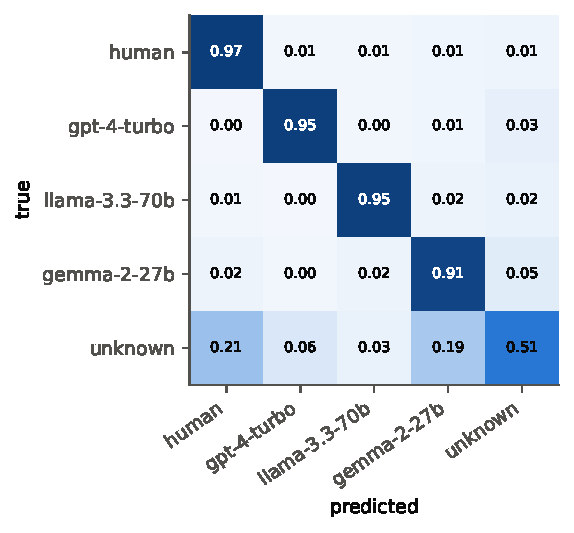
\includegraphics[width=0.55\linewidth]{figures/confusion.pdf}
\caption{Confusion matrix (row-normalised) of the hybrid detector with pseudo-unknown training on the development set.}
\label{fig:confusion}
\end{figure}

\subsection{Human vs.\ AI}
Table~\ref{tab:binary} collapses all generators into one class. All supervised detectors separate human and machine abstracts well (ROC-AUC 0.983--0.995), with mDeBERTa trained with pseudo-unknown data being the best (accuracy 0.9685, ROC-AUC 0.9946). Zero-shot detectors with Qwen3-0.6B are much weaker: 0.79 ROC-AUC for log-perplexity and 0.76 for Binoculars. We attribute this to the small observer model, the domain (Russian scientific prose has high perplexity even when written by a model) and the post-processing of the dataset; published Binoculars results use 7B models on English text.

\begin{table}[tbh!]
\begin{center}
\small
\begin{tabular}{|l|ccc|}
\hline
Method & Acc & F1 & ROC-AUC \\
\hline
Log-perplexity, zero-shot & 0.7677 & 0.8501 & 0.7892 \\
Binoculars, zero-shot & 0.7786 & 0.8656 & 0.7633 \\
TF-IDF + LR (official baseline) & 0.9378 & 0.9601 & 0.9861 \\
TF-IDF + LR (official baseline) + pseudo-unknown & 0.9443 & 0.9645 & 0.9867 \\
mDeBERTa-v3-base, fine-tuned & 0.9606 & 0.9755 & 0.9914 \\
mDeBERTa-v3-base, fine-tuned + pseudo-unknown & \textbf{0.9685} & \textbf{0.9805} & \textbf{0.9946} \\
Hybrid: emb + LM + style & 0.9305 & 0.9552 & 0.9826 \\
Hybrid: emb + LM + style + pseudo-unknown & 0.9454 & 0.9652 & 0.9868 \\
Hybrid: TF-IDF + emb + LM + style & 0.9212 & 0.9486 & 0.9827 \\
Hybrid: TF-IDF + emb + LM + style + pseudo-unknown & 0.9463 & 0.9656 & 0.9897 \\
Hybrid: TF-IDF + LM + style (ours) & 0.9279 & 0.9532 & 0.9862 \\
Hybrid: TF-IDF + LM + style (ours) + pseudo-unknown & 0.9478 & 0.9666 & 0.9896 \\
\hline
\end{tabular}

\caption{Human vs.\ AI on the development set (all five generator classes are ``AI''). Accuracy and F1 at the 0.5 threshold of $1-p(\text{human})$.}
\label{tab:binary}
\end{center}
\end{table}

\subsection{Ablation of the hybrid detector}
Table~\ref{tab:ablation} trains the hybrid classifier on subsets of the feature groups. Alone, the TF-IDF probabilities are the strongest group, and the e5 embeddings are the second (88.7\% on known classes). LM statistics and stylometry are weak on their own (65--67\%) but complementary: together they reach 75\%, and on top of TF-IDF each of them adds 0.7--0.9 pp on known classes and 4--5 pp of 5-class accuracy in the pseudo-unknown setting. Embeddings do not help on top of TF-IDF, and LightGBM is worse than logistic regression on the same features, so the final model is TF-IDF + LM + style with logistic regression. Its feature vector has only 30 dimensions, and training takes seconds.

\begin{table}[tbh!]
\begin{center}
\small
\begin{tabular}{|l|cc|cc|}
\hline
Feature groups & \multicolumn{2}{c|}{4 known classes} & \multicolumn{2}{c|}{+ pseudo-unknown} \\
 & Acc (4 known) & ROC-AUC & Acc (5 cl.) & Rec$_{unk}$ \\
\hline
TF-IDF & 0.9524 & 0.9849 & 0.8060 & 0.3139 \\
emb & 0.8872 & 0.9801 & 0.7481 & 0.2982 \\
LM & 0.6482 & 0.9138 & 0.5584 & 0.2697 \\
style & 0.6655 & 0.8823 & 0.5740 & 0.2706 \\
LM + style & 0.7508 & 0.9498 & 0.6455 & 0.3286 \\
emb + LM + style & 0.9163 & 0.9826 & 0.7806 & 0.3341 \\
TF-IDF + LM & 0.9595 & 0.9816 & 0.8474 & 0.4772 \\
TF-IDF + style & 0.9616 & 0.9862 & 0.8571 & \textbf{0.5186} \\
TF-IDF + LM + style & \textbf{0.9663} & \textbf{0.9862} & \textbf{0.8586} & 0.5067 \\
TF-IDF + emb + LM + style & 0.9617 & 0.9827 & 0.8379 & 0.4183 \\
emb + LM + style, LightGBM & 0.8865 & 0.9807 & -- & -- \\
\hline
\end{tabular}

\caption{Ablation of feature groups of the hybrid detector (logistic regression unless stated) on the development set. Left: trained on 4 known classes; right: trained with the pseudo-unknown class.}
\label{tab:ablation}
\end{center}
\end{table}

\subsection{How much do detectors rely on length?}
Table~\ref{tab:length} compares every method on full abstracts and on abstracts cut to 40 words (in training and in evaluation). All supervised methods lose 6--7 pp of accuracy on the known classes and 1--2 pp of ROC-AUC; the hybrid without TF-IDF, which depends more on stylometry, loses 10.5 pp, and zero-shot Binoculars loses 6.3 pp of ROC-AUC. The fine-tuned encoder is not more robust than the lexical baseline. The ranking of the methods does not change: the hybrid detector remains the best on known classes (90.5\%) and in the 5-class task (0.7686 vs.\ 0.7516 for mDeBERTa and 0.7262 for TF-IDF, all with their best unknown-class strategy).

\begin{table}[tbh!]
\begin{center}
\footnotesize
\begin{tabular}{|l|ccc|ccc|}
\hline
Method & \multicolumn{3}{c|}{Acc (4 known classes)} & \multicolumn{3}{c|}{Human vs AI ROC-AUC} \\
 & full & 40 words & $\Delta$, pp & full & 40 words & $\Delta$, pp \\
\hline
Binoculars, zero-shot & -- & -- & -- & 0.7633 & 0.7003 & -6.3 \\
TF-IDF + LR (official baseline) & 0.9523 & 0.8865 & -6.6 & 0.9861 & 0.9722 & -1.4 \\
TF-IDF + LR (official baseline) + pseudo-unknown & 0.9540 & 0.8855 & -6.8 & 0.9867 & 0.9734 & -1.3 \\
mDeBERTa-v3-base, fine-tuned & 0.9596 & 0.8960 & -6.4 & 0.9914 & 0.9806 & -1.1 \\
mDeBERTa-v3-base, fine-tuned + pseudo-unknown & 0.9564 & 0.8853 & -7.1 & 0.9946 & 0.9815 & -1.3 \\
Hybrid: emb + LM + style & 0.9163 & 0.8111 & -10.5 & 0.9826 & 0.9600 & -2.3 \\
Hybrid: TF-IDF + LM + style (ours) & 0.9663 & 0.9032 & -6.3 & 0.9862 & 0.9676 & -1.9 \\
Hybrid: TF-IDF + LM + style (ours) + pseudo-unknown & 0.9675 & 0.9045 & -6.3 & 0.9896 & 0.9741 & -1.6 \\
\hline
\end{tabular}

\caption{Length control: every model is retrained and evaluated on the first 40 words of each abstract. $\Delta$ is the change in percentage points.}
\label{tab:length}
\end{center}
\end{table}

Fig.~\ref{fig:buckets} gives a complementary view without retraining: ROC-AUC of models trained on full texts, computed separately for abstracts of different length. Short abstracts ($<$50 words), where 1{,}186 of the 1{,}766 AI texts are GigaChat-Lite and only 360 texts are human, are the hardest bucket for all methods. Above 50 words supervised detectors are almost perfect (ROC-AUC 0.98--1.00), including the 100+ bucket where AI texts are the minority. So length is a useful cue but not the only one: after removing most of it, about 90\% of known-class decisions are still correct.

\begin{figure}[!tbh]
\centering
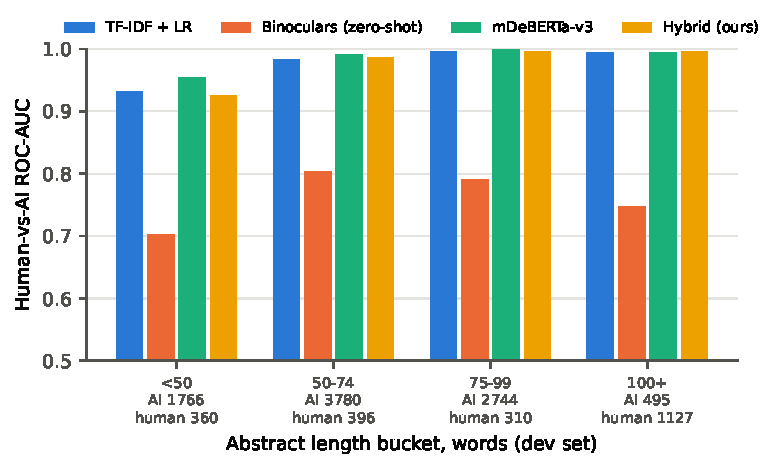
\includegraphics[width=0.8\linewidth]{figures/length_buckets.pdf}
\caption{Human-vs-AI ROC-AUC on the development set by abstract length (models trained on full texts, without pseudo-unknown data).}
\label{fig:buckets}
\end{figure}

\subsection{New generators}
Table~\ref{tab:heldout} evaluates the detectors on our held-out generations (topics taken from development-set abstracts; the human side are the same 947 human abstracts). As a binary detector, every supervised model catches practically all texts of the new generator(s): ROC-AUC is above 0.99 and the TPR at 5\% FPR is above 98\%. Zero-shot Binoculars is again weaker (0.91 ROC-AUC). The harder question is whether a model recognises the text as coming from an \emph{unknown} generator instead of attributing it to one of the known ones. Without pseudo-unknown data, mDeBERTa labels only 3\% of Qwen3-1.7B texts as unknown (3\% for YandexGPT) and the hybrid 15\% (13\% for YandexGPT); with pseudo-unknown data this rises to 48\% and 56\% for Qwen3-1.7B, and to 25\% and 67\% for YandexGPT. The hybrid detector generalises noticeably better than mDeBERTa to YandexGPT, a model from a different family than either pseudo-unknown generator, which suggests that its language-model and stylometric features capture something more general than \emph{which LLM family this is}.
A caveat is that Qwen3-1.7B belongs to the same family as one of our pseudo-unknown generators (Qwen3-4B), which makes it easier to recognise; YandexGPT-5-Lite is unrelated to any training generator and is the harder case of the two.

\begin{table}[tbh!]
\begin{center}
\small
\begin{tabular}{|l|ccc|ccc|}
\hline
Method & \multicolumn{3}{c|}{qwen3-1.7b} & \multicolumn{3}{c|}{yandexgpt-5-lite-8b} \\
 & ROC-AUC & TPR@5\% & Rec$_{unk}$ & ROC-AUC & TPR@5\% & Rec$_{unk}$ \\
\hline
Binoculars, zero-shot & 0.9086 & 0.6980 & -- & 0.8787 & 0.6103 & -- \\
TF-IDF + LR (official baseline) & 0.9954 & 0.9863 & 0.3643 & 0.9962 & 0.9894 & 0.2809 \\
TF-IDF + LR (official baseline) + pseudo-unknown & 0.9978 & 0.9937 & 0.5227 & 0.9962 & 0.9894 & 0.1172 \\
mDeBERTa-v3-base, fine-tuned & 0.9973 & 0.9989 & 0.0338 & 0.9978 & 0.9968 & 0.0348 \\
mDeBERTa-v3-base, fine-tuned + pseudo-unknown & \textbf{0.9985} & \textbf{1.0000} & 0.4752 & \textbf{0.9982} & \textbf{0.9979} & 0.2513 \\
Hybrid: TF-IDF + LM + style (ours) & 0.9963 & 0.9989 & 0.1478 & 0.9932 & 0.9884 & 0.1267 \\
Hybrid: TF-IDF + LM + style (ours) + pseudo-unknown & 0.9969 & \textbf{1.0000} & \textbf{0.5565} & 0.9948 & 0.9947 & \textbf{0.6684} \\
\hline
\end{tabular}

\caption{Held-out generators (never used in training), each paired with the same human abstracts. ROC-AUC and TPR@5\%FPR for human vs.\ AI; Rec$_{unk}$ is the share of generated texts predicted as ``unknown''.}
\label{tab:heldout}
\end{center}
\end{table}

\subsection{Output samples}
\begin{table}[!tbh]
\centering
\begin{tabular}{|p{0.64\linewidth}|l|l|}
\hline
Abstract (first 28 words) & Gold & Predicted \\
\hline
\parbox[t]{0.62\linewidth}{\raggedright\small Раскрывается правовое содержание дотаций как формы расходов бюджета. Для этого автор прослеживает, как рассчитывается уровень бюджетной обеспеченности субъекта РФ и что влияет на его определение. Обосновывается, что обязанность \dots} & human & human \\ \hline
\parbox[t]{0.62\linewidth}{\raggedright\small В данной статье уделяется внимание разбору ключевых физических процессов, происходящих в нижней хромосфере Солнца. Проанализирована взаимосвязь между фотосферой и хромосферой, что позволяет лучше понять их совместное влияние на \dots} & gpt-4-turbo & gpt-4-turbo \\ \hline
\parbox[t]{0.62\linewidth}{\raggedright\small Данная статья посвящена анализу инновационных подходов в строительстве скважин, направленных на повышение коэффициента нефтеотдачи и эффективности добычи углеводородов.} & unknown & unknown \\ \hline
\parbox[t]{0.62\linewidth}{\raggedright\small Статья описывает разработку метода ТБ-ИЗАТЕСТ на основе изотермической амплификации (LAMP), использующегося для диагностики Mycobacterium tuberculosis, возбудителя туберкулеза. Метод включает детекцию целевой последовательности ДНК гена rv2341 M. tuberculosis.} & unknown & gemma-2-27b \\ \hline
\parbox[t]{0.62\linewidth}{\raggedright\small Работа посвящена линейным непрерывным операторам, действующим в пространстве целых функций. Исследованы свойства таких операторов, связанные с определением операторов типа свертки в пространствах аналитических функций. Сформулированы следствия, уточняющие аппроксимационную \dots} & human & gemma-2-27b \\ \hline
\end{tabular}

\caption{Examples from the development set with the gold label and the prediction of the final hybrid detector (TF-IDF + LM + style, pseudo-unknown class). The last two rows are errors: a short GigaChat-Lite abstract attributed to Gemma-2 and a short human abstract attributed to Gemma-2.}
\label{tab:output}
\end{table}



\section{Conclusion}
We studied the detection of AI-generated Russian scientific abstracts on AINL-Eval 2025. We reproduced the official baseline, compared it with a fine-tuned mDeBERTa, zero-shot perplexity detectors and a hybrid feature-based detector, collected a new set of 6{,}595 abstracts generated by 2025 open LLMs with the official protocol, and ran a length-control study.

Main findings: (1) distinguishing the four known classes is almost solved (up to 96.8\% accuracy), and the difficulty of the task lies in the unknown generator; (2) simply adding generations of \emph{other} LLMs as a pseudo-unknown class improves 5-class accuracy by 5.5--6.2 pp for the neural and hybrid detectors, and our hybrid detector (TF-IDF stacking + Qwen3-0.6B statistics + stylometry, logistic regression) reaches 0.8586, which would rank third on the development leaderboard, behind two 7--8B LLM-based systems; (3) detectors do use the length of abstracts, but cutting texts to 40 words costs only 6--7 pp on known classes and does not change the ranking of the methods; (4) zero-shot detectors with small models are far behind supervised ones in this domain. The whole pipeline runs in under an hour on one GPU.

Limitations: results are from single runs; the private test set could not be used because its labels are not public; our held-out generators are few and partly related to the pseudo-unknown ones. Natural next steps are a larger pool of pseudo-unknown generators from different model families and zero-shot detectors with larger observer models.




\bibliographystyle{apalike}
\bibliography{lit}
\end{document}
